  Так как монитор светимости работает на базе электромагнитного калориметра, то полученные данные можно использовать для получения обратной связи с электромагнитным калориметром в режиме реального времени. Возможность получения обратной связи полезна тем, что можно оперативно обнаружить неисправности в работе электромагнитного калориметра и устранить их. В качестве обратной связи удобно использовать значения пьедесталов для каждого сектора. В общем случае пьедестал это отклонение уровня сигнала от нулевого положения?\par
  Для каждого из 32 секторов монитор светимости получает аналоговую сумму сигналов с 2 триггерных ячеек. Соответственно, имея форму сигнала, можно определять отклонение от нулевого положения для каждого сектора в режиме реально времени. Форма сигнала представляет собой массив из 2048 значений на один сектор. Расчет происходит следующим образом:
\begin{enumerate}
  \item Считываем формы сигналов с монитора светимости
  \item Находим максимальное значение в массиве
  \item Проверяем превышает ли максимальное значение установленное пороговое (устанавливаем было ли событие в данном секторе)
  \item Если максимальное значение превышает пороговое, то необходимо удалить 50 значений слева от максимума и 150 справа (Рис. 9). Иначе переходим к следующему пункту
  \item Считаем среднее арифметическое по оставшимся значениям
\end{enumerate}
Данный алгоритм повторяем для каждого сектора. Все полученые значения пьедесталов сохраняются в систему медленного контроля EPICS.
\begin{figure}[htp]
  \centering
  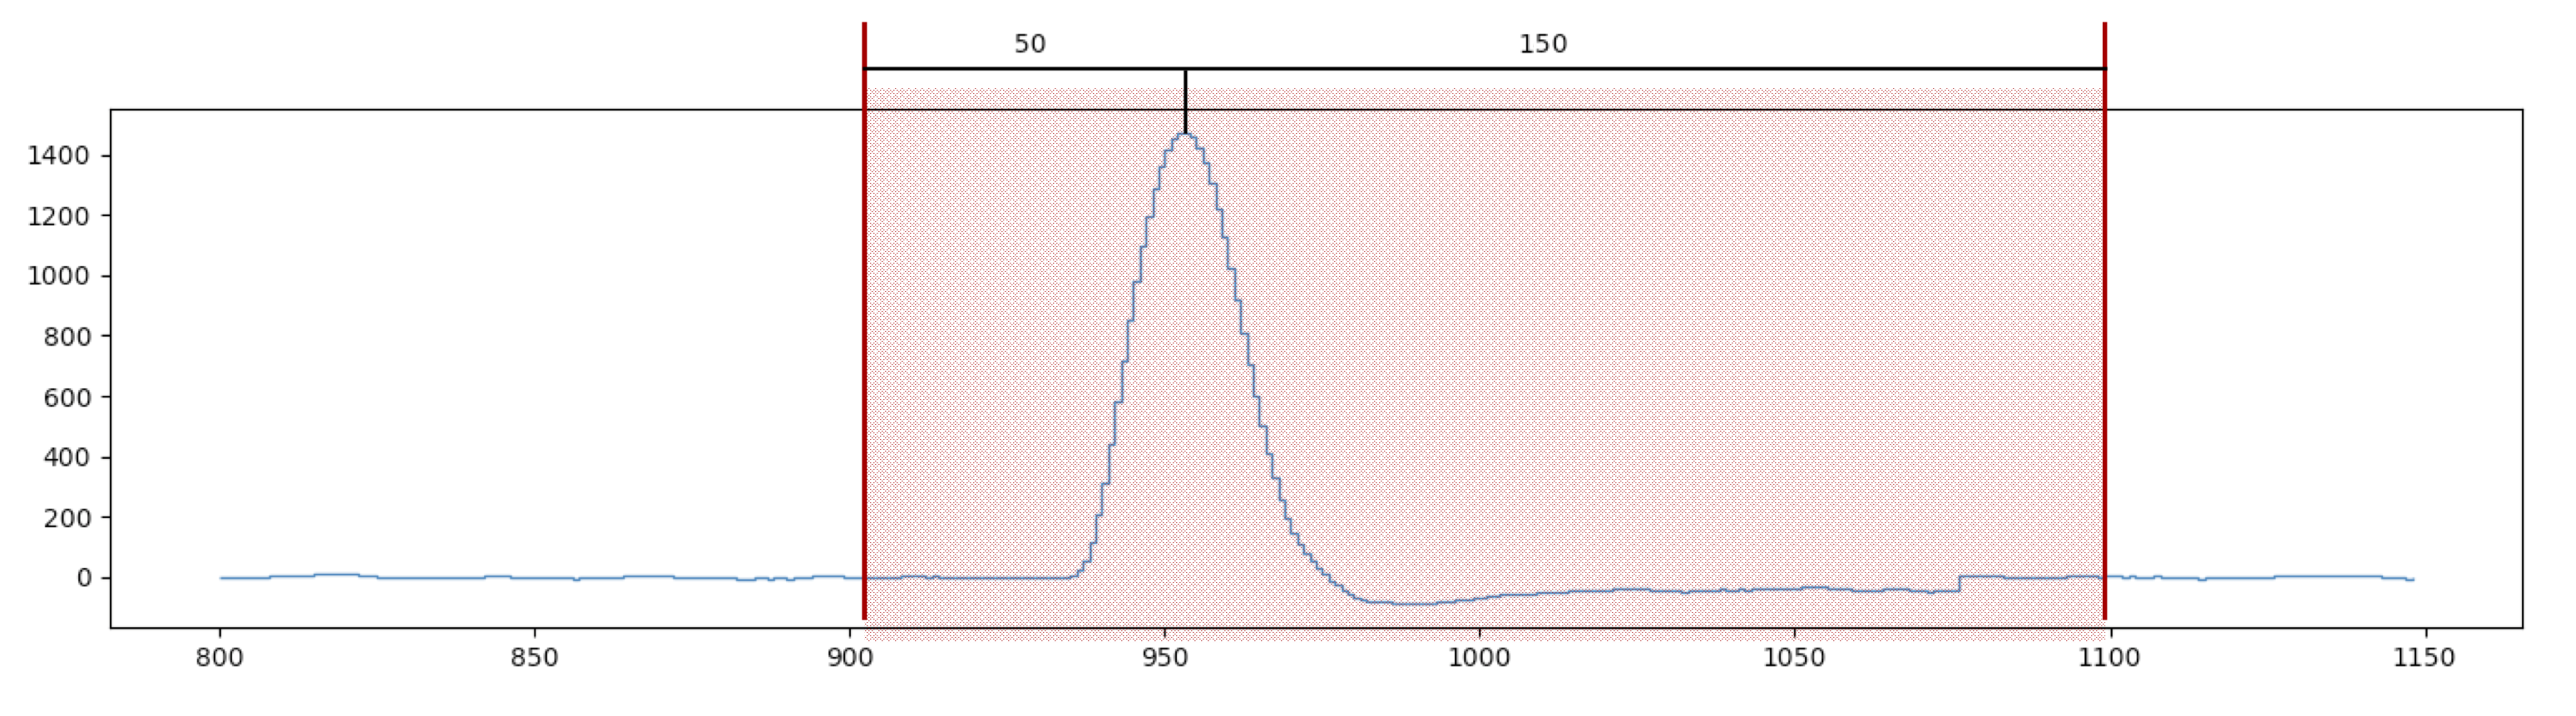
\includegraphics[width=\textwidth]{Pedestal}
  \caption{Схема расчета значений пьедесталов}
  \label{fig:galaxy}
\end{figure}
